\RequirePackage{plautopatch}
\documentclass[uplatex,dvipdfmx,paper=a4paper,fontsize=11pt,jafontscale=0.9247,lang=ja]{jlreq}

%=============================================
% パッケージ
%=============================================
\usepackage{geometry}
\usepackage{fancyhdr}
\usepackage{ascmac}
\usepackage{fancybox}
\usepackage{amsmath,amssymb}
\usepackage{array}
\usepackage{tabularx}
\usepackage{enumitem}
\usepackage{hhline}
\usepackage{otf}      % \ajMaru 用（uplatex必須）
\usepackage{xcolor}
\usepackage{multicol}
\usepackage{graphicx}
\usepackage{listings}
\usepackage{tcolorbox}
\usepackage{tikz}
\usepackage{calc}
\usepackage{otf}

\tcbuselibrary{skins,breakable,listings}

%=============================================
% レイアウト
%=============================================
\geometry{top=25mm,bottom=25mm,left=20mm,right=20mm}
\setlength{\headheight}{18pt}
\setlength{\headsep}{12pt}
\setlength{\footskip}{20pt}
\renewcommand{\figurename}{図}
%=============================================
% 共通テスト風 解答マクロ
%=============================================

% --- インライン解答欄 ---
\newcommand{\setanswer}[1]{\doublebox{\textbf{#1}}}

% --- 解答群のラベル ---
\newcommand{\answerlabel}[1]{\textbf{#1}~\textbf{の解答群}}

% --- ダミー定義 ---
\newcommand{\answerset}[1]{}

% --- answergroup (語句選択用) ---
% 引数1：列数（デフォルト3）
% 引数2：ラベル（a, b...）
% 引数3：中身（ 1... & 2... \\ ）
\newcommand{\answergroup}[3][3]{%
  \par\vspace{1em}\noindent
  \answerlabel{#2}\par
  \vspace{0.3em}\noindent
  \fbox{%
    \begin{minipage}{\dimexpr\linewidth-2\fboxsep-2\fboxrule\relax}
      \vspace{0.8em}
      \begin{tabularx}{\linewidth}{*{#1}{>{\raggedright\arraybackslash}X}}
        #3
      \end{tabularx}
      \vspace{0.4em}
    \end{minipage}%
  }
  \par\vspace{1em}
}

\newcommand{\answertable}[4]{%
  \par\vspace{1em}\noindent
  \answerlabel{#1}\par
  \vspace{0.3em}
  \noindent
  % 修正ポイント：1列目の右側の | を削除し、ループ側で補う
  \begin{tabular}{|c*{#2}{|c}|} 
    \cline{2-\numexpr#2+1\relax}
    \multicolumn{1}{c|}{} & #3 \\ \hline
    #4
  \end{tabular}
  \par\vspace{1em}
}

\newcommand{\dbox}[1]{%
  \begin{center}
    \begin{tikzpicture}
      \node[draw,dashed,inner sep=6pt,text width=0.95\linewidth, align=left]
      {#1};
    \end{tikzpicture}
  \end{center}
}
%=============================================
% 共通テスト風 会話環境
%=============================================
\newenvironment{dialogue}{%
  \begin{list}{}{%
    \setlength{\labelwidth}{3.5em} % ← 名前欄の幅（調整可）
    \setlength{\labelsep}{0.5em}
    \setlength{\leftmargin}{\labelwidth+\labelsep}
    \setlength{\itemindent}{0pt}
    \setlength{\listparindent}{0pt}
    \setlength{\parsep}{0pt}
  }
}{%
  \end{list}
}

% 話者コマンド
\newcommand{\speaker}[1]{\item[\textbf{#1：}]}

%=============================================
% 4. 問題階層マクロ
%=============================================
\newcommand{\daimon}[1]{\subsection*{#1}}
\newcommand{\syomon}[1]{\subsubsection*{#1}}
\newcommand{\komon}[1]{\textbf{#1}\quad}

%=============================================
% ページスタイル
%=============================================
\fancypagestyle{coverpage}{
  \fancyhf{}
  \cfoot{\small ―\ \thepage\ ―}
}

\fancypagestyle{instructionpage}{
  \fancyhf{}
  \cfoot{\small ―\ \thepage\ ―}
}

\fancypagestyle{exampage}{
  \fancyhf{}
  \lhead{\small 2026年度試験}
  \chead{\small 【第1回 Arcaea共通テスト】}
  \renewcommand{\headrulewidth}{0.4pt}
  \cfoot{\small ―\ \thepage\ ―}
  \rfoot{\small （次頁へ続く）}
  \renewcommand{\footrulewidth}{0.4pt}
}

\fancypagestyle{exampageend}{
  \lhead{\small 2026年度試験}
  \chead{\small 【第1回 Arcaea共通テスト】}
  \renewcommand{\headrulewidth}{0.4pt}
  \cfoot{\small ―\ \thepage\ ―}
  \rfoot{\small （試験問題は以上です）}
  \renewcommand{\footrulewidth}{0.4pt}
}

\fancypagestyle{acknowledgepage}{
  \fancyhf{}
}

%=============================================
% 科目開始・終了
%=============================================
\newcommand{\beginsubject}[1]{%
  \newpage
  \pagestyle{exampage}
  \rhead{#1}
  \begin{center}
    \vspace*{2em}
    {\LARGE\textbf{#1}}\\[0.5em]
    \rule{0.6\textwidth}{0.8pt}
  \end{center}
  \vspace{1em}
}

\newcommand{\finishsubject}{%
  \thispagestyle{exampageend}%
}

%=============================================
% 本文
%=============================================
\begin{document}
%===============================================
% 表紙
%===============================================
\thispagestyle{coverpage}
\begin{center}

\vspace*{3cm}

% 試験区分
\fbox{\parbox{0.85\textwidth}{
  \centering
  \vspace{0.8em}
  {\Large 2026年度}\\[1em]
  {\Huge\textbf{第1回　Arcaea共通テスト}}\\[1em]
  \vspace{0.8em}
}}

\vspace{3cm}

% 試験情報テーブル
\renewcommand{\arraystretch}{1.8}
\begin{tabular}{|>{\centering\arraybackslash}p{3.5cm}|>{\centering\arraybackslash}p{7cm}|}
\hline
\textbf{試験日} & 2026年　1月 10日（土） \\
\hline
\textbf{解答時間(目安)} & 60分 \\
\hline
\textbf{出題領域} & Arcaea・文科・理科 \\
\hline
\end{tabular}

\vspace{4cm}

\vspace{2cm}

% 主催
{\large 主催：tzug（$\mathbb{X}$ : @tzug\_c）}

\end{center}

%===============================================
%  注意事項ページ
%===============================================
\newpage
\thispagestyle{instructionpage}

\begin{center}
{\LARGE\textbf{注　意　事　項}}\\[0.5em]
\rule{0.7\textwidth}{1pt}
\end{center}

\vspace{1.5em}

\section*{1　試験全般について}
\begin{enumerate}
  \item 解答時間の目安は60分であるが，あくまで目安である．これを超えて解答してもよい．
  \item 解答は，すべて定められたフォームに記入すること．
  \item 問題については，すべて Ver 6.11.5 (2026/01/08)時点の情報に基づいて解答するものとし，それ以降の仕様変更等によらない．
\end{enumerate}

\section*{2　解答の形式について}
\begin{enumerate}
  \item 解答に際しては，必ず各問いにおいて指定された解答形式に従うこと．
  たとえば，答えが $2.5$ となる場合であっても，$\dfrac{5}{2}$ と記すよう指示されているときは，その指示に従うこと．
  
  \item $\dfrac{10}{4}$ や $2\sqrt{8}$ など，約分されていないものや，根号が簡約されていない形での解答は，正解と認められない．
  
  \item 分数型での解答を求められた場合，分数の符号は分子に付けること．
  
  \item 小数型での解答を求められた場合，指定された桁数の一つ下の桁を四捨五入して答えること．
  たとえば，$\fbox{キ}.\fbox{ク}\fbox{ケ}$ に $2.495$ と解答する場合は，$2.50$ と記入すること．
  
  \item 問題文中の二重四角で示された \doublebox{ナ} などの欄には，選択肢の中から最も適切なものを一つ選んで答えること．
\end{enumerate}

\section*{3　禁止事項}
\begin{enumerate}
  \item 解答の作成にあたり，生成AIを使用してはならない．
  
  \item 解答に直接結びつく行為を目的としない範囲に限り，用語や背景事項の確認のための検索エンジンの使用を認める．
\end{enumerate}

\section*{4　その他}
\begin{enumerate}
  \item 試験終了後における，本試験の感想や雰囲気等についての発信を妨げるものではない．広く歓迎する．
\end{enumerate}

\vfill
\begin{center}
\rule{0.5\textwidth}{0.4pt}\\[0.5em]
\end{center}

%===============================================
%  Arcaea
%===============================================
\beginsubject{A r c a e a}
\daimon{第1問}
次の各問いに答えよ．ただし，楽曲名横の[ ]内はその楽曲の難易度を表している．なお，[ ]内のPST，PRS，FTR，ETR，BYDはそれぞれPAST，PRESENT，FUTURE，ETERNAL，BEYONDの略記である．
日本語表記，外国語表記は，ゲーム内言語設定に基づくものとする．
\answerset{0}% カウンタをリセット（アから開始）※ダミー定義によりエラー回避
\begin{enumerate}[label=(\arabic*)]
\item 次のうち，Arcaeaのパートナーである光，対立，紅の英語表記で，正しい組み合わせは \doublebox{a} である．
\answertable{\doublebox{a}}{4}{ \ajMaru{0} & \ajMaru{1} & \ajMaru{2} & \ajMaru{3} }{
    光& Light      & Lux & Hikari & Hikari \\ 
    対立 & Conflict & Conflictus & Tairitsu &Tairitsu \\
    紅 & Crimson    & Vermiculus & Kou& Beni\\ \hline
}

\item 次のうち，同じ楽曲名が複数存在するものは \doublebox{b} である(コラボ楽曲を含む)．
\answergroup[4]{\doublebox{b}}{
  \textcircled{\scriptsize 0} Quon & 
  \textcircled{\scriptsize 1} Temptation & 
  \textcircled{\scriptsize 2} GLORY : ROAD & 
  \textcircled{\scriptsize 3} Jingle
}

\item 次のうち，現在の譜面難易度レベルが10+であるものは \doublebox{c} である.
\answergroup[2]{\doublebox{c}}{
  \textcircled{\scriptsize 0} Singularity[FTR] & 
  \textcircled{\scriptsize 1} Axium Crisis[FTR] \\ 
  \textcircled{\scriptsize 2} Tempestissimo[FTR] & 
  \textcircled{\scriptsize 3} \#1f1e33[FTR]
}
\item 次のうち，Arcaeaに存在しない楽曲名は \doublebox{d} である．
\answergroup[2]{\doublebox{d}}{
  \textcircled{\scriptsize 0} Quon & 
  \textcircled{\scriptsize 1} これでホントにサヨナラ \\
  \textcircled{\scriptsize 2} Aether Crest: Celestial & 
  \textcircled{\scriptsize 3} Vulc\={a}nus 
  }
\newpage
\item Grievous LadyのPAST，PRESENT，FUTURE譜面製作者として正しい組み合わせは，次のうち \doublebox{e} である．
\answertable{\doublebox{e}}{4}{ \ajMaru{0} & \ajMaru{1} & \ajMaru{2} & \ajMaru{3} }{
    PAST     & 迷路上層 & 迷路表層 & 迷路第一層 & 迷路第一層  \\ 
    PRESENT  & 迷路中層 & 迷路中層 & 迷路第二層 & 迷路第二層 \\
    FUTURE   & 迷路下層 & 迷路深層 & 迷路第三層 & 迷路深層\\ \hline
}
\item 次の図\ref{fig:basic}と図\ref{fig:advance}はそれぞれ基本編と応用編のゲームチュートリアルの画面である．
    それぞれの曲名($\alpha$)，($\beta$)と，その作曲者($\gamma$)の組み合わせとして正しいものは \doublebox{f} である．
    \begin{figure}[h]
        \centering
        \begin{minipage}[b]{0.49\columnwidth}
            \centering
            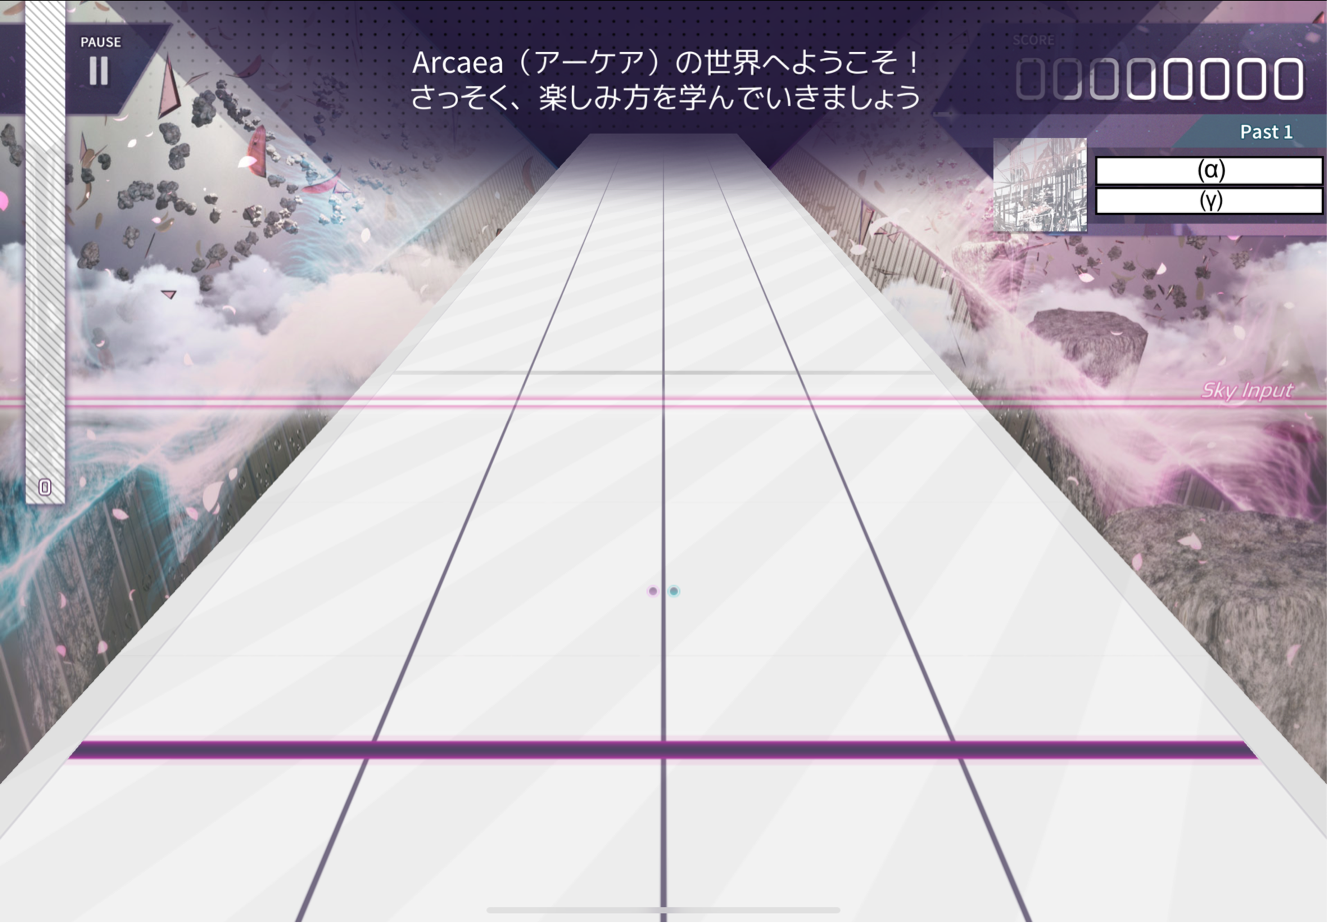
\includegraphics[width=0.9\columnwidth]{../images/tex/tutorial_q.png}
            \caption{基本編のチュートリアル}
            \label{fig:basic}
        \end{minipage}
        \begin{minipage}[b]{0.49\columnwidth}
            \centering
            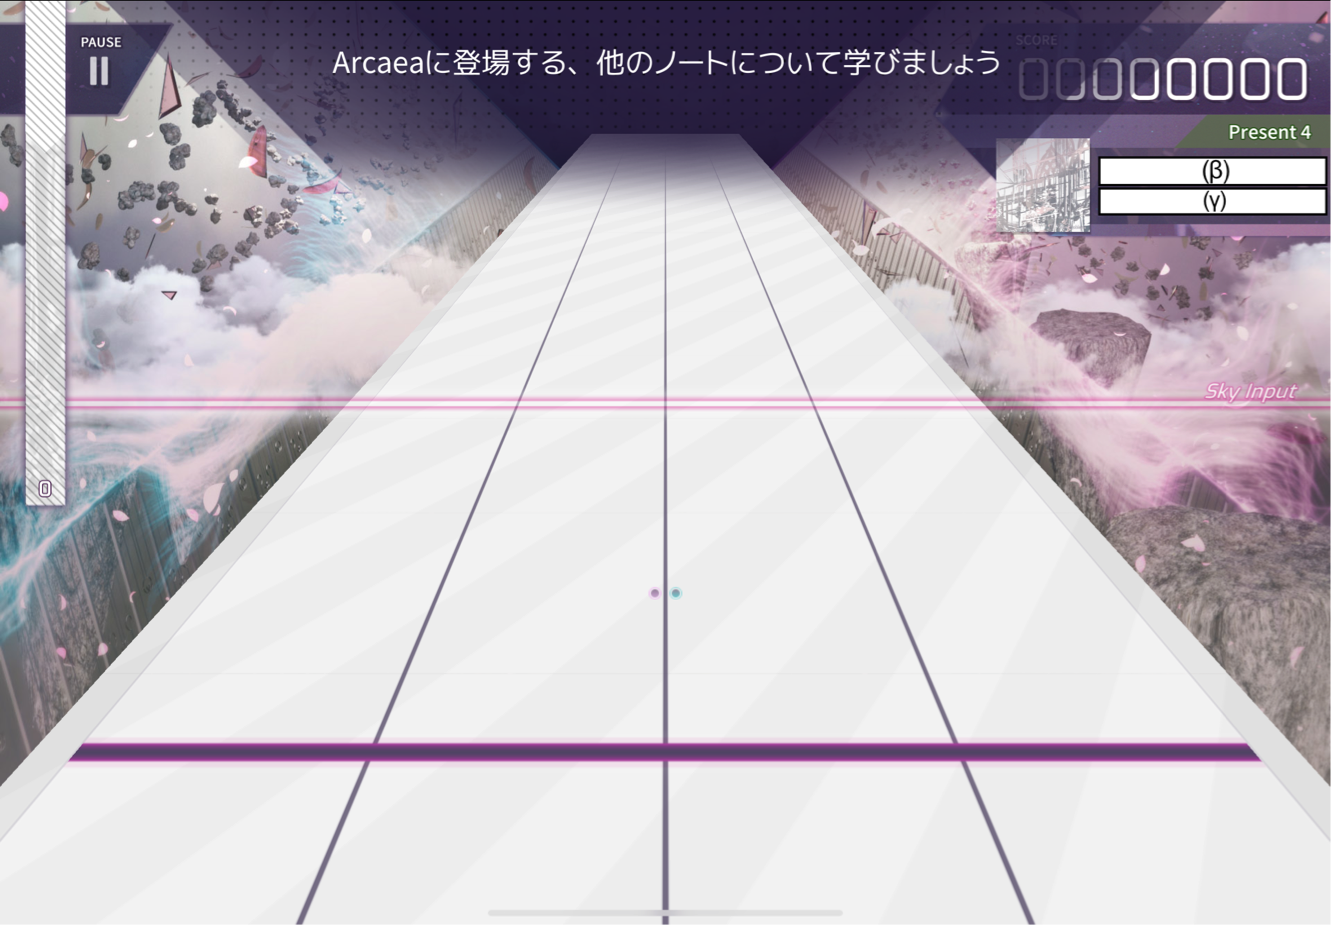
\includegraphics[width=0.9\columnwidth]{../images/tex/ad-tutorial_q.png}
            \caption{応用編のチュートリアル}
            \label{fig:advance}
        \end{minipage}
    \end{figure}
    \answertable{\doublebox{f}}{4}{ \ajMaru{0} & \ajMaru{1} & \ajMaru{2} & \ajMaru{3} }{
    ($\alpha$) & Tutorial          & Tutorial          & Tutorial $\mathrm{I}$  & Tutorial $\mathrm{I}$  \\ 
    ($\beta$)  & Advanced Tutorial & Advanced Tutorial & Tutorial $\mathrm{II}$ & Tutorial $\mathrm{II}$ \\
    ($\gamma$) & ak+q              & Tutorial          & ak+q        & Tutorial    \\ \hline
}
\newpage
\item 次のパートナーは，Side Storyのとあるパートナーである．以下の各問いに答えよ．
\begin{figure}[h]
    \centering
    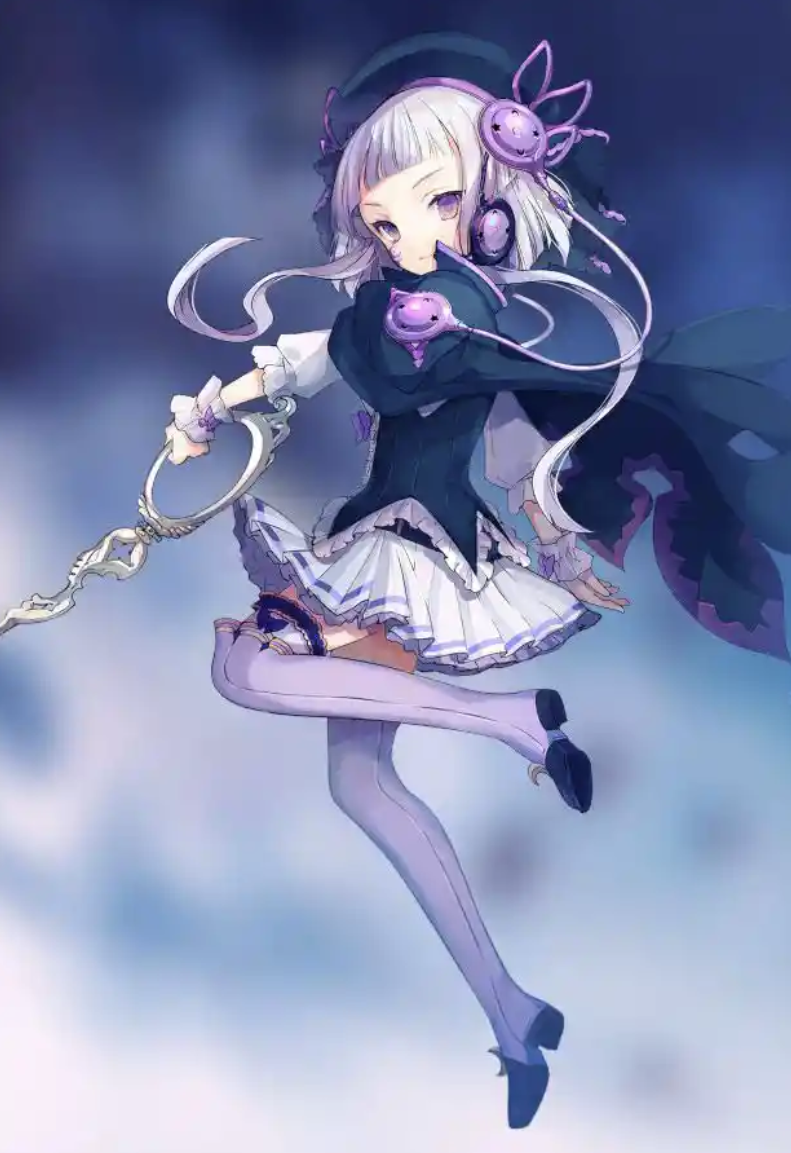
\includegraphics[width=0.35\columnwidth]{../images/tex/runa.png}
    \caption{とあるパートナー}
    \vspace{-0.5em} % キャプションと出典の間の距離を詰める
    {\footnotesize （出典　https://wikiwiki.jp/arcaea/　より引用，一部改変）}
    \label{fig:runa}
\end{figure}
\\
    \begin{enumerate}[label=(\roman*)]
        \item このパートナーの名前は \doublebox{g} で，このパートナーを選択して楽曲をプレイすると， \doublebox{h} ．
        \answergroup[4]{\doublebox{g}}{
            \textcircled{\scriptsize 0} エト&
            \textcircled{\scriptsize 1} ルナ&
            \textcircled{\scriptsize 2} 奈実&
            \textcircled{\scriptsize 3} 天々音
          }
          \answergroup[1]{\doublebox{h}}{
            \textcircled{\scriptsize 0} 「光」サイド楽曲をプレイした時，得られる欠片の数が+5される\\
            \textcircled{\scriptsize 1} 「対立」サイド楽曲をプレイした時，得られる欠片の数が+5される\\
            \textcircled{\scriptsize 2} FAR判定が非表示になる\\
            \textcircled{\scriptsize 3} 想起率が非表示になる
          }
          \newpage
        \item このパートナーの入手方法についての説明で，最も適切なものは，次のうち \doublebox{i} である．
        \answergroup[1]{\doublebox{i}}{
            \textcircled{\scriptsize 0} Binary Enfoldを購入すると即座に解放されるWorld mapを進めると入手できる． \\
            \textcircled{\scriptsize 1} ある条件下で楽曲「Singularity」をクリアすると解禁されるWorld mapを進めると入手できる．\\
            \textcircled{\scriptsize 2} 楽曲「Singularity」を入手すると，即座に入手できる．\\
            \textcircled{\scriptsize 3} このパートナーの姉を覚醒させると，このパートナーへ変更可能になる．
          }
    \end{enumerate}
\newpage
\item 次のパートナーは，とある期間限定パートナーである．以下の各問いに答えよ．
\begin{figure}[h]
    \centering
    
\includegraphics[width=0.35\columnwidth]{../images/tex/midsummer-kanae.png}
    \caption{とあるパートナー}
    \vspace{-0.5em} % キャプションと出典の間の距離を詰める
    {\footnotesize （出典　https://wikiwiki.jp/arcaea/　より引用，一部改変）}
    \label{fig:kanae}
\end{figure}
\\
    \begin{enumerate}[label=(\roman*)]
        \item このパートナーの名前として最も適切なものは，次のうち \doublebox{j} である．
        \answergroup[4]{\doublebox{j}}{
            \textcircled{\scriptsize 0} サマー 叶 & 
            \textcircled{\scriptsize 1} 盛夏 叶\\
            \textcircled{\scriptsize 2} サマー 叶永 & 
            \textcircled{\scriptsize 3} 盛夏 叶永 
        }
        \item このパートナーのスキルについての説明で，最も適切なものは，次のうち \doublebox{k} である．
        \answergroup[1]{\doublebox{k}}{
            \textcircled{\scriptsize 0} 昼間と夜間の区別によって，スキル効果が変化する． \\
            \textcircled{\scriptsize 1} プレイヤーの位置情報や，時間以外の地理的条件によって，スキル効果が変化する．\\
            \textcircled{\scriptsize 2} 午前と午後の区別によって，スキル効果が変化する．\\
            \textcircled{\scriptsize 3} 1年の前期と後期の区別によって，スキル効果が変化する．
          }
    \end{enumerate}
    \newpage
    \item Arcaea Song Contest 2020入賞曲として，「HIVEMIND」という楽曲がある．以下の各問いに答えよ．
    \begin{enumerate}[label=(\roman*)]
        \item HIVEMIND[PST]の譜面の特徴として，最も適切なものは次のうち \doublebox{l} である．
        \answergroup[1]{\doublebox{l}}{
            \textcircled{\scriptsize 0} 他の譜面と同様に，フロア・ロング・スカイ・アークノーツから構成されている．\\ 
            \textcircled{\scriptsize 1} 他の譜面と違い，ロング・スカイ・アークノーツのみから構成されている．\\
            \textcircled{\scriptsize 2} 他の譜面と違い，フロア・スカイノーツのみから構成されている．\\
            \textcircled{\scriptsize 3} 他の譜面と違い，ロング・アークノーツのみから構成されている． 
        }
        \item HIVEMIND[FTR]の譜面の特徴として，最も適切なものは次のうち \doublebox{m} である．
        \answergroup[1]{\doublebox{m}}{
            \textcircled{\scriptsize 0} 他の譜面と同様に，フロア・ロング・スカイ・アークノーツから構成されている．\\
            \textcircled{\scriptsize 1} 他の譜面と違い，ロング・スカイ・アークノーツのみから構成されている．\\
            \textcircled{\scriptsize 2} 他の譜面と違い，フロア・スカイノーツのみから構成されている．\\
            \textcircled{\scriptsize 3} 他の譜面と違い，ロング・アークノーツのみから構成されている． 
        }
    \end{enumerate}
\end{enumerate}
% 例:
% \subsection*{第1問}
% 問題内容...

\vfill
\newpage

\vfill
%===============================================
%  文科
%===============================================
\beginsubject{文　科}
% 頻出漢字，漢字の読み，
\daimon{第1問}
\begin{enumerate}[label=(\arabic*)]
    \item 次の表1〜7は，ArcaeaのAct $\mathrm{I}$ストーリーに登場する漢字を，出現回数の多い順にまとめたものである．
    表1はAct $\mathrm{I}$全文を対象とし，表2〜7は，Act $\mathrm{I}$の各章（Eternal CoreからFinal Verdictまで）をそれぞれ対象として調べた結果を，順不同に並べたものである．
    ただし，第0章は対象に含まれない．
    また，本問では，「1-1」や「F-4」のような表記を，それぞれ第1章第1話，第F章第4話と読むものとする．
    ここで，章名とは「Eternal Core」，「Final Verdict」などを指し，「1-2」や「F-7」における「1」や「F」にあたる部分を章番号という．
    章番号は順序を表す記号であり，その大小関係は Act $\mathrm{I}$ におけるストーリーの進行順に従って定義する．
    例えば第1章は第VS章より前であり，第F章は第VS章の後にある．
    
    以下の各問いに答えよ．
    \newpage
    \begin{table}
        \centering
        \caption{Act \protect$\mathrm{I}$ 中に登場する漢字}
        \vspace{0.5em}
    \begin{tabular}{|c c|} \hline
        漢字& 回数 \\ \hline
        \doublebox{1} & 635 \\ %女
        \doublebox{2} & 374 \\ %少
        \doublebox{3} & 249 \\ %彼
        \doublebox{4} & 236 \\ %光
        \doublebox{5} & 226 \\ %片
        \doublebox{6} & 219 \\ %見
        \doublebox{7} & 213 \\ %一
        \doublebox{8} & 211 \\ %硝
        \doublebox{9} & 206 \\ %界
        \doublebox{10} & 192 \\ \hline %世
      \end{tabular}
    \end{table}
    \begin{table}[htbp]
        \centering
        \begin{minipage}{0.32\linewidth}
            \centering
            \caption{\protect\doublebox{13}}%Vicious Labyrinth
            \begin{tabular}{|c c|} \hline
            \doublebox{1} & 79 \\ %女
            \doublebox{2} & 60 \\ %少
            \doublebox{11} & 31 \\ %憶
            \doublebox{12} & 30 \\ %記
            \doublebox{9} & 28 \\ \hline %界
            \end{tabular}
            \end{minipage}
        \hfill
        \begin{minipage}{0.32\linewidth}
            \centering
            \caption{\protect\doublebox{14}}%Luminous Sky
            \begin{tabular}{|c c|} \hline
            \doublebox{1} & 73 \\ %女
            \doublebox{3} & 44 \\ %彼
            \doublebox{2} & 29 \\ %少
            自 & 27 \\ %自
            \doublebox{5} & 24 \\ \hline %片
            \end{tabular}
            \end{minipage}
        \hfill
        \begin{minipage}{0.32\linewidth}
            \centering
            \caption{\protect\doublebox{15}} %Eternal Core
            \begin{tabular}{|c c|} \hline
            \doublebox{1} & 35 \\ %女
            \doublebox{5} & 33 \\ %片
            \doublebox{2}，\doublebox{8} & 30 \\ %少，硝
            \doublebox{11}，\doublebox{12} & 23 \\ %記，憶
            \doublebox{9}，\doublebox{10} & 15\\ \hline %世，界
            \end{tabular}
            \end{minipage}
        \end{table}
        \begin{table}[htbp]
        \centering
        \begin{minipage}{0.32\linewidth}
            \centering
            \caption{\protect\doublebox{16}} %Final Verdict
            \begin{tabular}{|c c|} \hline
            \doublebox{1} & 235 \\ %女
            \doublebox{2} & 152 \\ %少
            \doublebox{9} & 112 \\ %界
            \doublebox{10} & 102 \\ %世
            \doublebox{7} & 100 \\ \hline %一
            \end{tabular}
            \end{minipage}
        \hfill
        \begin{minipage}{0.32\linewidth}
            \centering
            \caption{\protect\doublebox{17}} %Adverse Prelude
            \begin{tabular}{|c c|} \hline
            \doublebox{1} & 102 \\ %女
            \doublebox{2} & 55 \\ %少
            \doublebox{3} & 51 \\ %彼
             自& 38 \\ %自
            \doublebox{6} & 34 \\ \hline %見
            \end{tabular}
            \end{minipage}
        \hfill
        \begin{minipage}{0.32\linewidth}
            \centering
            \caption{\protect\doublebox{18}}%Black Fate
            \begin{tabular}{|c c|} \hline
            \doublebox{1} & 100 \\ %女
            \doublebox{8} & 77 \\ %硝
            \doublebox{4} & 73 \\ %光
            \doublebox{5} & 72 \\ %片
            \doublebox{3} & 67 \\ \hline %彼
        \end{tabular}
        \end{minipage}
        \end{table}
        \newpage
    \begin{enumerate}[label=(\roman*)]
        \item ~\doublebox{1} - \doublebox{12}に当てはまる漢字を，次のメモ1を参考にしながら，以下の解答群から選べ．
        \begin{itembox}[l]{\textbf{メモ1}}
        \begin{itemize}
            \item \doublebox{2} と \doublebox{8}は，共通の音読みを一つ持っている．
            \item \doublebox{5}，\doublebox{8}，\doublebox{9}，\doublebox{10}，\doublebox{11}，\doublebox{12} は，特定の単語に対し独自の読み「Arcaea」が振られることがある．
            \item \doublebox{6}\doublebox{7}という熟語がAct $\mathrm{I}$ の中で少なくとも1回は登場する．
            \item Act $\mathrm{I}$ 前半では，光と対立がそれぞれ探索を重ねながら，物語が進行する．
        \end{itemize}
        \end{itembox}
        \answergroup[5]{\doublebox{1} - \doublebox{12}}{
            \textcircled{\scriptsize 0}  男&
            \textcircled{\scriptsize 1}  女&
            \textcircled{\scriptsize 2}  対&
            \textcircled{\scriptsize 3}  立&
            \textcircled{\scriptsize 4}  光\\
            \textcircled{\scriptsize 5}  記&
            \textcircled{\scriptsize 6}  追&
            \textcircled{\scriptsize 7}  憶&
            \textcircled{\scriptsize 8}  佳&
            \textcircled{\scriptsize 9}  人\\
            \textcircled{\scriptsize 10} 少&
            \textcircled{\scriptsize 11} 氏&
            \textcircled{\scriptsize 12} 奴&
            \textcircled{\scriptsize 13} 彼&
            \textcircled{\scriptsize 14} 小\\
            \textcircled{\scriptsize 15} 欠&
            \textcircled{\scriptsize 16} 片&
            \textcircled{\scriptsize 17} 子&
            \textcircled{\scriptsize 18} 硝&
            \textcircled{\scriptsize 19} 一\\
            \textcircled{\scriptsize 20} 見&
            \textcircled{\scriptsize 21} 三&
            \textcircled{\scriptsize 22} 千&
            \textcircled{\scriptsize 23} 世&
            \textcircled{\scriptsize 24} 界
        }
        \item ~\doublebox{13} - \doublebox{18}に対応する章名を，次のメモ2を参考にしながらそれぞれ選べ．
        \begin{itembox}[l]{\textbf{メモ2}}
            \begin{itemize}
                \item \doublebox{14} は \doublebox{13}の前にある．
                \item \doublebox{17} の章番号は「V」である．
            \end{itemize}
            \end{itembox}
        \answergroup[3]{\doublebox{13} - \doublebox{18}}{
            \textcircled{\scriptsize 0} Eternal Core&
            \textcircled{\scriptsize 1} Luminous Sky\\
            \textcircled{\scriptsize 2} Vicious Labyrinth&
            \textcircled{\scriptsize 3} Adverse Prelude\\
            \textcircled{\scriptsize 4} Black Fate&
            \textcircled{\scriptsize 5} Final Verdict
        }
        \item 第0章中に，\doublebox{2} は \doublebox{19} 回登場する．
        \answergroup[4]{\doublebox{19}}{
            \textcircled{\scriptsize 0} 1&
            \textcircled{\scriptsize 1} 11&
            \textcircled{\scriptsize 2} 23&
            \textcircled{\scriptsize 3} 47\\
        }
    \end{enumerate}
\end{enumerate}
\vfill
\newpage
% %===============================================
%  理科
%===============================================
\beginsubject{理　科}
% RSA暗号(双子素数と素因数分解など)、階段の問題
% ここに問題を記入
\daimon{第1問}

光さんと対立さんは，Arcaeaに収録されている楽曲「Nhelv」のBPM（テンポ）について話している．
二人の会話を読み，下の問い（問1～3）に答えよ．

\vspace{1em}
\dbox{
\begin{dialogue}
  \speaker{光}
  「Nhelv」のBPM表示を見たんだけど，\textbf{174.59} だって．どうしてこんなに中途半端な値になっているんだろう？

  \speaker{対立}
  この曲，独特な音程のズレを感じるわね．電子音楽の制作手法の一つに，曲全体の再生速度を変更することで，音の高さ（ピッチ）とテンポを同時に変化させる手法があるわ．

  \speaker{光}
  なるほど．レコードやカセットテープの回転数を変えるようなものだね．再生速度を落とせば， 音高は \doublebox{ア} ，テンポは \doublebox{イ} ね．

  \speaker{対立}
  ええ．実はこの曲がとある音楽ゲームに最初に収録されたときのBPMは \textbf{175.89} とされているの．もし，作曲者が「キリの良いBPM」で作った後に，意図的に「音高を微調整」した結果だとしたら，元のBPMを計算で割り出せるかもしれないわ．

  \speaker{光}
  面白そう！ 音高の変化量とBPMの変化比率は比例するはずだから，数学的に逆算できそうだね．
\end{dialogue}
}
\begin{enumerate}[label=(\arabic*)]
\item 会話文中の\doublebox{ア}，\doublebox{イ}に入る適切な語をそれぞれ選べ．
\answergroup[3]{\doublebox{ア}}{%2
  \textcircled{\scriptsize 0} 高くなり &
  \textcircled{\scriptsize 1} 変わらず &  
  \textcircled{\scriptsize 2} 低くなり
}
\answergroup[3]{\doublebox{イ}}{%1
  \textcircled{\scriptsize 0} 速くなる & 
  \textcircled{\scriptsize 1} 変わらない & 
  \textcircled{\scriptsize 2} 遅くなる
}

\newpage
\item
再生速度の変化比 $R$ と，音程の変化$n$ の関係は，以下の式で近似できることが知られている．
\[
R = 2^{\frac{n}{12}}
\]
ここで，$n$ は半音単位での変化量を表し，音高が上がるときに正の値をとる．
「Nhelv」では，制作段階から \textbf{0.4半音} 音高を下げているという情報がある．
このとき，再生速度の変化比 $R$ の値として最も適切なものは \doublebox{ウ} である．
\begin{table}[h]
  \centering
  \caption{半音変化数 $n$ と $2^{\frac{n}{12}}$ の値}
  \label{tab:route2}
  \begin{tabular}{|c||c|c|c|c|c|c|} \hline
    $n$ & $-0.5$ & $-0.4$ & $-0.3$ & $0.3$ &$0.4$ & $0.5$ \\ \hline
    $2^{\frac{n}{12}}$ & $0.971532$ & $0.977160$ & $0.982821$ & $1.01748$ &$1.02337$ & $1.02930$ \\ \hline
  \end{tabular}
\end{table}

\answergroup[3]{\doublebox{ウ}}{%1
  \textcircled{\scriptsize 0} $0.971532$ & 
  \textcircled{\scriptsize 1} $0.977160$ &
  \textcircled{\scriptsize 2} $0.982821$ \\
  \textcircled{\scriptsize 3} $1.01748$ &
  \textcircled{\scriptsize 4} $1.02337$ & 
  \textcircled{\scriptsize 5} $1.02930$
}
\item
前問で選んだ比率 $R$ を用いて，変更前の「元のBPM」を推測する．
変更後のBPMが $175.89$ であるとき，変更前のBPM $X$ は次の方程式で表される．
\[
X \times R = 175.89
\]
この式と(2)の値を用いれば，元のBPM $X$ は
$\fbox{エオカ}.\fbox{キク}$%180.00
である．
\newpage
\item
二人は，再生速度の変化比 $R$ と周波数（音の高さ）の関係についてさらに考察を深めた．

\vspace{1em}
\dbox{
\begin{dialogue}
  \speaker{対立}
    再生速度を $R$ 倍にすると，単位時間あたりに送出される波の数も $R$ 倍になるわ。つまり，元の周波数を $f_0$，変化後の周波数を $f$ とすると，$f = R \times f_0$ が成り立つわね。
  \speaker{光}
    そうだね。じゃあ、元の周波数 $f_0$ を固定して、半音の変化数 $n$ を変数としたときの周波数 $f$ の変化をグラフに表すとどうなるだろう。
\end{dialogue}
}

\begin{enumerate}[label=(\roman*)]
%=============================================
% グラフ選択問題
%=============================================
\item 
    下図は，半音の変化数 $n$ と周波数 $f$ の関係を表したグラフの概形である．
    このグラフとして最も適当なものは，次のうち \doublebox{ケ} である．なお，以下のグラフはすべて線形目盛上に描かれている．

    \vspace{1em}
    \doublebox{ケ}\textbf{の解答群}
    \vspace{1em}

    % --- 行ベースの配置 (0,1 / 2,3 / 4,5) ---
    \noindent
    \begin{minipage}[t]{0.48\linewidth}
    \centering
    % --- 選択肢 0 : 正答（指数関数的増加・下に凸・切片あり） ---
    \textcircled{\scriptsize 0}\\[0.5em]
    \begin{tikzpicture}[scale=0.6, baseline=(current bounding box.center)]
        \draw[->,>=stealth] (-0.5,0) -- (4,0) node[right] {$n$};
        \draw[->,>=stealth] (0,-0.5) -- (0,4) node[above] {$f$};
        \node[left] at (0,1.2) {\small $f_0$};
        \draw[thick] (-0.1, 1.2) -- (0.1, 1.2);
        % y = 1.2 * exp(0.35x)
        \draw[domain=0:3.2, smooth, variable=\x, thick] plot ({\x}, {1.2*exp(0.35*\x)});
        \node[below left] at (0,0) {O};
    \end{tikzpicture}
    \end{minipage}
    \hfill
    \begin{minipage}[t]{0.48\linewidth}
    \centering
    % --- 選択肢 1 : 比例誤認（直線・切片あり） ---
    \textcircled{\scriptsize 1}\\[0.5em]
    \begin{tikzpicture}[scale=0.6, baseline=(current bounding box.center)]
        \draw[->,>=stealth] (-0.5,0) -- (4,0) node[right] {$n$};
        \draw[->,>=stealth] (0,-0.5) -- (0,4) node[above] {$f$};
        \node[left] at (0,1.2) {\small $f_0$};
        \draw[thick] (-0.1, 1.2) -- (0.1, 1.2);
        % y = 1.2 + 0.8x
        \draw[thick] (0, 1.2) -- (3.2, 3.76); 
        \node[below left] at (0,0) {O};
    \end{tikzpicture}
    \end{minipage}

    \vspace{1.5em}

    \noindent
    \begin{minipage}[t]{0.48\linewidth}
        \centering
        % --- 選択肢 2 : 対数誤認（上に凸・切片あり） ---
        \textcircled{\scriptsize 2}\\[0.5em]
        \begin{tikzpicture}[scale=0.6, baseline=(current bounding box.center)]
            \draw[->,>=stealth] (-0.5,0) -- (4,0) node[right] {$n$};
            \draw[->,>=stealth] (0,-0.5) -- (0,4) node[above] {$f$};
            \node[left] at (0,1.2) {\small $f_0$};
            \draw[thick] (-0.1, 1.2) -- (0.1, 1.2);
            % y = 1.2 + 1.5 * ln(x + 1)
            \draw[domain=0:3.5, smooth, variable=\x, thick] plot ({\x}, {1.2 + 1.5*ln(\x + 1)});
            \node[below left] at (0,0) {O};
        \end{tikzpicture}
    \end{minipage}
    \hfill
    \begin{minipage}[t]{0.48\linewidth}
        \centering
        % --- 選択肢 3 : 定数誤認（水平） ---
        \textcircled{\scriptsize 3}\\[0.5em]
        \begin{tikzpicture}[scale=0.6, baseline=(current bounding box.center)]
            \draw[->,>=stealth] (-0.5,0) -- (4,0) node[right] {$n$};
            \draw[->,>=stealth] (0,-0.5) -- (0,4) node[above] {$f$};
            \node[left] at (0,1.2) {\small $f_0$};
            \draw[thick] (-0.1, 1.2) -- (0.1, 1.2);
            % y = 1.2 (constant)
            \draw[thick] (0, 1.2) -- (3.5, 1.2);
            \node[below left] at (0,0) {O};
        \end{tikzpicture}
    \end{minipage}

    \vspace{1.5em}

    \noindent
    \begin{minipage}[t]{0.48\linewidth}
        \centering
        % --- 選択肢 4 : 切片忘れ（原点通過・指数関数・枠一杯に修正） ---
        \textcircled{\scriptsize 4}\\[0.5em]
        \begin{tikzpicture}[scale=0.6, baseline=(current bounding box.center)]
            \draw[->,>=stealth] (-0.5,0) -- (4,0) node[right] {$n$};
            \draw[->,>=stealth] (0,-0.5) -- (0,4) node[above] {$f$};
            % 修正: 係数を調整して x=3.5 付近で y=4 近くまで伸びるように変更
            % y = 0.05 * exp(1.25 * x)
            \draw[domain=0:3.5, smooth, variable=\x, thick] plot ({\x}, {0.05*exp(1.25*\x)});
            \node[below left] at (0,0) {O};
        \end{tikzpicture}
    \end{minipage}
    \hfill
    \begin{minipage}[t]{0.48\linewidth}
        \centering
        % --- 選択肢 5 : 離散誤認（階段状） ---
        \textcircled{\scriptsize 5}\\[0.5em]
        \begin{tikzpicture}[scale=0.6, baseline=(current bounding box.center)]
            \draw[->,>=stealth] (-0.5,0) -- (4,0) node[right] {$n$};
            \draw[->,>=stealth] (0,-0.5) -- (0,4) node[above] {$f$};
            \node[left] at (0,1.2) {\small $f_0$};
            \draw[thick] (-0.1, 1.2) -- (0.1, 1.2);
            % Step function
            \draw[thick] (0, 1.2) -- (0.8, 1.2) -- (0.8, 1.6) -- (1.6, 1.6) -- (1.6, 2.1) -- (2.4, 2.1) -- (2.4, 2.7) -- (3.2, 2.7);
    \node[below left] at (0,0) {O};
\end{tikzpicture}
\end{minipage}
    \vspace{1em}
\newpage
    \item 
    会話は続く。
    \dbox{
    \begin{dialogue}
      \speaker{光}
        なるほどね．この式を $\log_2$ を使って書き直すと，$n = \doublebox{コ} \times \log_2 \left( \frac{f}{f_0} \right)$ になるね．
      \speaker{対立}
        ええ．この式から，周波数が $2$ 倍になると音高がちょうど $12$ 半音（1オクターブ）上がることが数学的にも説明できるわ．
    \end{dialogue}
    }
    \answergroup[4]{\doublebox{コ}}{
      \textcircled{\scriptsize 0} $1$ & \textcircled{\scriptsize 1} $6$ & \textcircled{\scriptsize 2} $12$ & \textcircled{\scriptsize 3} $24$
    }
    元の楽曲（BPM $\fbox{エオカ}.\fbox{キク}$）の基準となる「ラ」の音が $440$ Hz であったとしよう．
    制作段階でピッチを $0.4$ 半音下げた場合，変化後の「ラ」の周波数は $\fbox{サシス} Hz$である．必要ならば表\ref{tab:route2}の値を参照せよ．
\end{enumerate}
\end{enumerate}
\newpage

\daimon{第2問}
光さんと対立さんは，在りし日は豪邸に続いていたであろう螺旋階段を上っている．
二人は気を紛らわせるために，階段の上り方が何通りあるかを数えながら進むことにした．
以下の会話を読み，次の各問いに答えよ．

\vspace{1em}
\dbox{
\begin{dialogue}
  \speaker{対立}
    ……はぁ．また，この階段．終わりが見えないわね．
  \speaker{光}
    そうだね．ただ上っているだけだと気が滅入っちゃうから，上り方のパターンを数えながら進んでみない？
  \speaker{対立}
    ……物好きなことね．でも，ただ歩くよりは退屈しのぎにはなるかしら．
  \speaker{光}
    ルールは簡単だよ．\textbf{「1段上る」}か\textbf{「1段飛ばし（一気に2段上る）」}のどちらかで進んでいくことにしよう．
  \speaker{対立}
    分かったわ．例えば，3段目まで上るなら，
    \begin{itemize}
        \item 1段，1段，1段
        \item 1段，2段
        \item 2段，1段
    \end{itemize}
    の3通りの方法があるということね．
\end{dialogue}
}

\begin{enumerate}[label=(\arabic*)]
\item このルールの下で，4段目まで上る方法は全部で \fbox{セ} 通りである．

\vspace{1em}

\item 会話は続く．
\dbox{
\begin{dialogue}
  \speaker{対立}
    いちいち書き出すのは効率が悪いわ．$n$ 段目まで上る方法の総数を $a_n$ として，関係式を作りましょう．
  \speaker{光}
    $n$ 段目（$n \geqq 3$）に到達する直前の一歩は，「1段上る」か「2段上る」のどちらかだよね．
  \speaker{対立}
    ええ．つまり，$a_n$ は $a_{n-1}$ と $a_{n-2}$ を用いて表せるわ．
\end{dialogue}
}

\begin{enumerate}[label=(\roman*)]
\item $n \geqq 3$ のとき，数列 $\{a_n\}$ について，正しい関係式を表しているものは \doublebox{ソ} である．

\answergroup[2]{\doublebox{ソ}}{
  \textcircled{\scriptsize 0} $a_n = a_{n-1} + a_{n-2}$ & 
  \textcircled{\scriptsize 1} $a_n = 2a_{n-1} + a_{n-2}$ \\
  \textcircled{\scriptsize 2} $a_n = a_{n-1} + 2a_{n-2}$ & 
  \textcircled{\scriptsize 3} $a_n = a_{n-1} \times a_{n-2}$
}
\newpage
\item 会話は続く．

\dbox{
\begin{dialogue}
  \speaker{対立}
    この漸化式を解くために，式変形をしましょう．
    定数 $p, q$ を用いて，
    \[ a_n - p a_{n-1} = q ( a_{n-1} - p a_{n-2} ) \] %a_n - p a_{n-1} = q ( a_{n-1} - p a_{n-2} )
    という形に変形できれば，これは「公比 \doublebox{タ} の等比数列」と見なせるわ．%q
  \speaker{光}
    なるほど．この式を展開して整理すると
    \[ a_n = (p+q) a_{n-1} - pq a_{n-2} \] %a_n = (p+q) a_{n-1} - pq a_{n-2}
    になるね．
  \speaker{対立}
    ええ．この式が元の漸化式 \doublebox{ソ} と一致すればいいのよ．
\end{dialogue}
} 
係数を比較することで，$p, q$ は和が $1$，積が $-1$ であることがわかる．
解と係数の関係により，$p, q$ は $x$ についての2次方程式
\[ x^2 - x - 1 = 0 \]
の2つの解であることが導かれる．この2つの解を $\alpha, \beta$ ($\alpha > \beta$) とおく．
\answergroup[2]{\doublebox{タ}}{
  \textcircled{\scriptsize 0} $p$ & 
  \textcircled{\scriptsize 1} $q$ 
}
\newpage

\begin{enumerate}[label=(\alph*)]
    \item
上の変形を利用すると，一般項 $a_n$ を求めることができる．
$a_n - \beta a_{n-1}$ は初項 $a_2 - \beta a_1$，公比 $\alpha$ の等比数列であるから，
\[ a_n - \beta a_{n-1} = (a_2 - \beta a_1) \alpha^{n-2} \]
ここで，具体的な数値 $a_1=1, a_2=2$ を代入し，同様に $a_n - \alpha a_{n-1}$ についても考えると，
$a_n$ は $\alpha, \beta$ を用いて次のように表される．

\[ a_n = \frac{ \alpha^{\text{\tiny\doublebox{ツ}}} - \beta^{\text{\tiny\doublebox{ツ}}} }{ \doublebox{チ} } \] %{n+1} 

\answergroup[4]{\doublebox{チ}}{
  \textcircled{\scriptsize 0} $\alpha - \beta$ & %0
  \textcircled{\scriptsize 1} $\alpha + \beta$ &
  \textcircled{\scriptsize 2} $\alpha \beta$ & 
  \textcircled{\scriptsize 3} $2$ 
}

\answergroup[5]{\doublebox{ツ}}{
  \textcircled{\scriptsize 0} $n-2$ & %0
  \textcircled{\scriptsize 1} $n-1$ &
  \textcircled{\scriptsize 2} $n$ & 
  \textcircled{\scriptsize 3} $n+1$ &
  \textcircled{\scriptsize 4} $n+2$ 
}

なお，$\alpha = \dfrac{\fbox{ト}+\sqrt{\fbox{ナ}}}{\fbox{テ}}$ は黄金比と呼ばれている．
\end{enumerate}
\end{enumerate}
\newpage
\item 
会話は続く．

\vspace{1em}
\dbox{
\begin{dialogue}
  \speaker{光}
    はぁ，はぁ……．ずっと2段上りとかしてると，やっぱり疲れちゃうね．
  \speaker{対立}
    無駄な動きが多いのよ．……でも，確かに足に来るわね．
  \speaker{光}
    じゃあ，ルールを少し変えよう．さっきの動きに加えて，\textbf{「2段上りを，2回以上連続で行うことはできない」}という制限をつけようよ．これなら少しは楽になるかも．
  \speaker{対立}
    条件が変われば，計算式も変わるわね．この新ルールの下で，$n$ 段目まで上る方法の総数を $b_n$ としましょう．
\end{dialogue}
}

新ルールの下では，例えば3段目までの上り方は問1のときと変わらず3通り（$b_3=3$）だが，
4段目までの上り方は，問1で挙げた方法のうち「2段，2段」という動きが禁止されるため， $\fbox{キ}-1$ 通りとなる．

\begin{enumerate}[label=(\roman*)]
    \item $n \geqq 4$ のとき，数列 $\{b_n\}$ には，\doublebox{ニ} という関係が成り立つ．
    \answergroup[2]{\doublebox{ニ}}{
    \textcircled{\scriptsize 0} $b_n = b_{n-1} + b_{n-2}$ & 
    \textcircled{\scriptsize 1} $b_n = b_{n-1} + b_{n-3}$ \\
    \textcircled{\scriptsize 2} $b_n = b_{n-1} + b_{n-2} - b_{n-3}$ & 
    \textcircled{\scriptsize 3} $b_n = b_{n-1} \times b_{n-3}$
    }
    \item 新ルールのもと，16段目まで上る方法 $b_{16}$ は \fbox{ヌネノ} 通りである．
    \item $b_{616}$ を$2$で割ったあまりは \fbox{ハ} である．
\end{enumerate}

\vspace{2em}
\end{enumerate}
\vfill
\finishsubject
\end{document}